\documentclass[12pt,a4paper,oneside]{report}

% ============================================================
% PACKAGES
% ============================================================
\usepackage[a4paper,margin=1in]{geometry}
\usepackage{graphicx}
\usepackage{float}
\usepackage{array}
\usepackage{longtable}
\usepackage{tabularx}
\usepackage{booktabs}
\usepackage{enumitem}
\usepackage{xcolor}
\usepackage{setspace}
\usepackage{titlesec}
\usepackage{fancyhdr}
\usepackage[hidelinks]{hyperref}
\usepackage{caption}
\usepackage{multirow}
\usepackage{ragged2e}
\usepackage{url}
\usepackage{xcolor}
\definecolor{skyblue}{RGB}{70,160,220}
\usepackage{fancyhdr}

\fancypagestyle{projectstyle}{
    \fancyhf{}
    \fancyhead[R]{\textbf{Ai Based Synthetic Media Detection System}}
    \renewcommand{\headrulewidth}{0.4pt}

    \fancyfoot[L]{Department of AI \& DS Engineering}
    \fancyfoot[R]{Page | \thepage}
    \renewcommand{\footrulewidth}{0.4pt}
}

% ============================================================
% GENERAL SETTINGS
% ============================================================
\onehalfspacing

\setlength{\parindent}{0pt}
\setlength{\parskip}{6pt}

\renewcommand{\contentsname}{INDEX}
\renewcommand{\listfigurename}{FIGURE INDEX}

% Chapter formatting
\titleformat{\chapter}
    {\normalfont\bfseries\Large\centering}
    {}
    {0pt}
    {}

\titleformat{\section}
    {\normalfont\bfseries\large}
    {\thesection}
    {0.5em}
    {}

\titleformat{\subsection}
    {\normalfont\bfseries\normalsize}
    {\thesubsection}
    {0.5em}
    {}

% Header and footer
\pagestyle{fancy}
\fancyhf{}
\fancyfoot[C]{\thepage}

% ============================================================
% DOCUMENT
% ============================================================
\begin{document}

% ============================================================
% COVER / PROJECT INFORMATION PAGE
% ============================================================
\begin{titlepage}

\thispagestyle{projectstyle}
\centering

\vspace*{-0.90cm}

{\Large\bfseries
Matoshri College of Engineering and Research Centre, Eklahare, Nashik.}

\vspace{-0.12cm}

{\large\bfseries
Department Of Artificial Intelligence \& Data Science Engineering
}

\vspace{-0.12cm}

{\large\bfseries
Project Synopsis
}

\vspace{0.35cm}

\renewcommand{\arraystretch}{1.22}
\setlength{\tabcolsep}{5pt}

\begin{tabular}{|p{7.0cm}|p{10.0cm}|}
\hline
\textbf{Title of Project Dissertation} &
\textbf{Ai Based Synthetic Media Detection System} \\
\hline

\textbf{Branch and Faculty} &
Faculty of Science \& Technology \\
\hline

\textbf{Name of College} &
Matoshri College of Engineering \& Research Centre, Nashik \\
\hline

\textbf{Name of the Students} &
\begin{tabular}{@{}ll@{}}
1. Ruturani Maske & 2. Gayatri Ahire \\
3. Kajal Kasar & 4. Sakshi Salve
\end{tabular}
\\
\hline

\textbf{PRN No.} &
\begin{tabular}{@{}ll@{}}
1. 72248390C & 2. 72248140D \\
3. 72248336J & 4. 72248494B
\end{tabular}
\\
\hline

\textbf{Email ID} &
\begin{tabular}{@{}l@{}}
1. ruturanimaske123@gmail.com \\
2. ahiregayatri889@gmail.com \\
3. kasarkajal972@gmail.com \\
4. sakshisalve891@gmail.com
\end{tabular}
\\
\hline

\textbf{Mobile Number} &
\begin{tabular}{@{}ll@{}}
1. 9156848403 & 2. 9834745763 \\
3. 9373385274 & 4. 7447571944
\end{tabular}
\\
\hline

\textbf{College PUN Code} &
\\[0.25cm]
\hline

\textbf{College Code} &
\\[0.25cm]
\hline

\textbf{Sign of the Student} &
1. \hspace{1.7cm} 2. \hspace{1.7cm} 3. \hspace{1.7cm} 4. \\
[0.35cm]
\hline

\textbf{Name of the Guide} &
\textbf{Dr. Ranjit M. Gawande} \\
\hline

\textbf{Sign of the Guide} &
\\[0.35cm]
\hline

\textbf{Name of the Project Coordinator} &
Mr. Mahesh T. Dhande \\
\hline

\textbf{Name of the Head of Department} &
Dr. Ranjit M. Gawande \\
\hline

\textbf{Sign of the Head of Department} &
\\[0.35cm]
\hline

\textbf{Date of Submission} &
\\[0.25cm]
\hline

\end{tabular}

\vfill

{\large\bfseries
Academic Year: 2026--2027
}

\vspace{0.15cm}

\end{titlepage}


% ============================================================
% SYNOPSIS TITLE PAGE
% ============================================================
\begin{titlepage}

\begin{center}

\vspace*{-1cm}

{\Large\bfseries
SYNOPSIS
}

\vspace{0.5cm}

{\large
of
}

\vspace{0.5cm}

{\LARGE\bfseries
PROJECT TITLE
}

\vspace{0.4cm}

{\Large\bfseries
Ai Based Synthetic Media Detection System
}

\vspace{0.1cm}

{\large
by
}

\vspace{0.2cm}

\begin{tabular}{c}
\textcolor{skyblue}{\textbf{Ruturani Maske (72248390C)}} \\[0.2cm]
\textcolor{skyblue}{\textbf{Gayatri Ahire (72248140D)}} \\[0.2cm]
\textcolor{skyblue}{\textbf{Kajal Kasar (72248336J)}} \\[0.2cm]
\textcolor{skyblue}{\textbf{Sakshi Salve (72248494B)}}
\end{tabular}

\vspace{1cm}

{\large
Under the guidance of
}

\vspace{0.3cm}

{\large
\textcolor{skyblue}{\textbf{Dr. Ranjit M. Gawande}}
}

\vspace{0.3cm}

{\large
in
}

\vspace{0.3cm}

{\large
partial fulfilment of the degree of
}

\vspace{0.3cm}

{\large\bfseries
Bachelor of Artificial Intelligence \& Data Science Engineering
}

\vspace{0.6cm}

{\large
Matoshri College of Engineering and Research Centre, Nashik
}

\vspace{0.1cm}

{\large
Department of Artificial Intelligence \& Data Science Engineering
}

\vspace{0.4cm}

{\large
Under
}

\vspace{0.3cm}


\includegraphics[width=4.5cm]{logo.png}

\vspace{0.3cm}

{\large\bfseries
Savitribai Phule Pune University, Pune
}

\vfill

{\large\bfseries
2026--2027
}

\end{center}

\end{titlepage}


% ============================================================
% INDEX
% ============================================================
\tableofcontents
\clearpage


% ============================================================
% FIGURE INDEX
% ============================================================
\listoffigures
\clearpage


% ============================================================
% ACKNOWLEDGEMENT
% ============================================================
\chapter*{ACKNOWLEDGEMENT}
\addcontentsline{toc}{chapter}{ACKNOWLEDGEMENT}

I express my heartfelt gratitude towards \textbf{ Dr. Ranjit M. Gawande}, Project Guide at Matoshri College of Engineering \& Research Centre, Nashik, for providing valuable guidance, encouragement, and continuous support throughout the development of the project dissertation entitled \textbf{``Ai Based Synthetic Media Detection System''}.

I humbly thank \textbf{Dr. Ranjit M. Gawande}, Head of the Department of Artificial Intelligence \& Data Science Engineering, for his valuable guidance and support throughout this project.

I am also thankful to \textbf{Mr. Mahesh T. Dhande}, Project Coordinator, and all the faculty members and staff of MCOERC, Nashik, for their valuable suggestions, technical support, and encouragement during the project work.

I would also like to express my sincere gratitude to the Principal and management of Matoshri College of Engineering and Research Centre, Nashik, for providing the necessary facilities and academic environment required for completing this work.

Finally, I express my sincere thanks to my family members, friends, and colleagues who directly or indirectly supported and encouraged me throughout the development of this project.

\vspace{1.5cm}

\begin{flushright}
\begin{tabular}{c}
\textbf{Ruturani Maske (72248390C)} \\[0.2cm]
\textbf{Gayatri Ahire (72248140D)} \\[0.2cm]
\textbf{Kajal Kasar (72248336J)} \\[0.2cm]
\textbf{Sakshi Salve (72248494B)}
\end{tabular}
\end{flushright}


% ============================================================
% ABSTRACT
% ============================================================
\chapter*{Abstract}
\addcontentsline{toc}{chapter}{Abstract}

The rapid advancement of artificial intelligence has made it possible to generate highly realistic manipulated facial images, commonly known as deepfakes. These images can be difficult to identify through manual inspection and may affect digital trust, privacy, security, and information authenticity. \textbf{Ai Based Synthetic Media Detection System} is proposed as an AI-based web application for detecting whether an uploaded facial image is real or manipulated. The system performs image preprocessing and face detection before applying a deep learning model for Real/Fake classification. It provides a confidence score and explainable analysis using Grad-CAM and heatmap visualization. The application also provides a result dashboard, detection history, report generation, user authentication, database storage, and an administrator dashboard. The system is implemented using Flask with HTML, CSS, and JavaScript. The proposed solution aims to provide an accessible, user-friendly, and explainable platform for preliminary deepfake image analysis.

\vspace{0.4cm}

\textbf{Keywords:} Deepfake Detection, Artificial Intelligence, Deep Learning, Face Detection, Grad-CAM, Explainable AI, Image Classification, Computer Vision, Flask.


% ============================================================
% CHAPTER 1
% ============================================================
\chapter{Introduction}
\pagestyle{projectstyle}
\thispagestyle{projectstyle}

% Introduction content

Deepfake technology represents a significant development in artificial intelligence-based media generation and manipulation. Deep learning techniques can be used to modify facial identities, expressions, and visual characteristics, resulting in synthetic content that can appear highly realistic. The increasing quality and accessibility of these technologies make the identification of manipulated content an important challenge in digital media forensics.

Deepfake detection systems generally analyze visual patterns, facial characteristics, texture inconsistencies, frequency information, blending artifacts, or other learned representations to distinguish genuine content from manipulated content. Research has demonstrated that deep learning-based approaches can effectively detect facial manipulations, although generalization to unseen manipulation techniques remains a major challenge.

The proposed \textbf{Ai Based Synthetic Media Detection System} system focuses on image-based facial deepfake detection. A user can upload an image through a web interface, after which the system performs preprocessing and face detection. The detected facial information is provided to a deep learning classification model that predicts whether the input is Real or Fake.

In addition to classification, the proposed system provides a confidence score and explainability through Grad-CAM/heatmap visualization. This enables the user to understand which image regions contributed to the model prediction. The system also maintains detection history, generates reports, and provides separate user and administrator functionalities.

The application uses Flask as the backend framework and HTML, CSS, and JavaScript for the frontend. A database is used for authentication, user records, detection history, and related results.

% ------------------------------------------------------------
\section{Existing System}

Existing deepfake detection approaches primarily focus on developing machine learning and deep learning models that classify manipulated and genuine facial content. Several methods use convolutional neural networks, frequency-domain information, facial artifacts, local relationships, or specialized image representations.

Although these approaches can achieve strong performance on benchmark datasets, many systems are primarily research-oriented and do not provide an integrated user-facing application. Users may need technical knowledge to execute models, prepare datasets, interpret outputs, or analyze detection results.

Another limitation is that many deep learning detectors operate as black-box classifiers. They may provide a prediction without clearly showing which regions of an image influenced the decision. Therefore, there is a need for a practical detection platform that combines classification with explainability and user-oriented functionality.

% ------------------------------------------------------------
\section{Significance and Background}

Deepfake detection is significant because manipulated facial images can be used for misinformation, impersonation, fraud, identity manipulation, unauthorized content generation, and other forms of digital abuse.

The background of this project lies in the application of artificial intelligence, computer vision, deep learning, and explainable artificial intelligence to digital media verification. A practical detection system should not only classify an image but should also communicate the result in an understandable form.

Ai Based Synthetic Media Detection System addresses this requirement by combining automated facial analysis with confidence scoring and visual explanation.

% ------------------------------------------------------------
\section{Scope}

The scope of the proposed system includes:

\begin{itemize}
    \item Detection of deepfake facial images.
    \item Face detection from uploaded images.
    \item Real/Fake classification.
    \item Confidence score generation.
    \item Deepfake analysis.
    \item Grad-CAM and heatmap visualization.
    \item Result dashboard.
    \item Detection history.
    \item Detection report generation.
    \item User authentication and login.
    \item Database management.
    \item Administrator dashboard.
    \item User-friendly web-based interface.
\end{itemize}

% ------------------------------------------------------------
\section{Limitations}

The proposed system has the following limitations:

\begin{itemize}
    \item The system is primarily focused on image-based deepfake detection.
    \item Detection performance depends on the quality and diversity of the training dataset.
    \item Highly sophisticated or previously unseen manipulation techniques may reduce detection reliability.
    \item Poor-quality, heavily compressed, blurred, or partially occluded images may affect detection performance.
    \item The confidence score represents model confidence and should not be treated as absolute proof of authenticity.
    \item The system is intended as an automated preliminary analysis tool rather than a replacement for professional forensic investigation.
\end{itemize}

% ------------------------------------------------------------
\section{Proposed System}

The proposed Ai Based Synthetic Media Detection System system provides an integrated web-based platform for analyzing facial images.

The system accepts an uploaded image and performs preprocessing and face detection. The detected facial region is then analyzed by a deep learning model. The model generates a Real/Fake prediction and confidence score.

For improved interpretability, Grad-CAM/heatmap visualization is generated to indicate image regions that contributed to the model decision. The result dashboard presents the prediction, confidence score, analysis, detected face, and visualization.

The system stores detection information in a database, allowing users to access previous detection records. Reports can also be generated from the detection results. Authentication mechanisms provide secure access, while the administrator dashboard enables system monitoring and management.

% ------------------------------------------------------------
\section{Advantages of Proposed System}

\begin{itemize}
    \item Automated deepfake image detection.
    \item Face-based image analysis.
    \item Real/Fake classification.
    \item Confidence score for predictions.
    \item Explainable prediction using Grad-CAM/heatmap.
    \item User-friendly web interface.
    \item Detection history management.
    \item Report generation.
    \item Secure user authentication.
    \item Persistent database storage.
    \item Administrator monitoring and management.
    \item Centralized detection workflow.
\end{itemize}


% ============================================================
% CHAPTER 2
% ============================================================
\chapter{Literature Survey}

Deepfake detection has developed rapidly with the advancement of deep learning and generative artificial intelligence. Existing research has explored CNN-based classifiers, manipulation-specific detection, generalizable facial forgery detection, local feature relationships, and explainable forensic analysis.

Rössler et al. introduced FaceForensics++, a large-scale benchmark for facial manipulation detection containing multiple manipulation techniques and different compression levels. The work demonstrated the importance of standardized datasets and domain-specific knowledge for automated facial forgery detection.

Li et al. proposed Face X-Ray, an image representation designed to identify blending boundaries in forged facial images. The method aims to improve generalization by focusing on intrinsic blending evidence rather than relying solely on artifacts associated with a particular manipulation technique.

Chen et al. proposed Local Relation Learning for Face Forgery Detection. Their method considers relationships among local facial regions using multi-scale patch similarity and combines RGB and frequency-domain information. The work highlights the importance of local relationships and frequency information for robust facial forgery detection.

Tariq et al. investigated general deepfake detection through a generalized framework and emphasized the problem of transferability and generalization to unseen deepfake generation methods. Their CLRNet approach combines spatial and temporal information to improve generalization.

Silva et al. proposed an explainable hierarchical ensemble for deepfake forensics. Their approach combines deep learning detection with explainable analysis and Grad-CAM, demonstrating the value of providing interpretable information alongside automated predictions.

These studies indicate that deepfake detection requires not only strong classification performance but also generalization, interpretability, and practical usability. The proposed Ai Based Synthetic Media Detection System system builds upon these concepts by integrating deepfake classification, face detection, confidence scoring, Grad-CAM/heatmap visualization, and a complete web-based management interface.

% ============================================================
% 2.1 SUMMARY TABLE OF SURVEY
% ============================================================
\section{Summary Table of Survey}

\renewcommand{\arraystretch}{1.20}
\setlength{\tabcolsep}{2pt}

\begin{longtable}{|
>{\raggedright\arraybackslash}p{0.55cm}|
>{\raggedright\arraybackslash}p{0.65cm}|
>{\raggedright\arraybackslash}p{2.30cm}|
>{\raggedright\arraybackslash}p{1.55cm}|
>{\raggedright\arraybackslash}p{2.05cm}|
>{\raggedright\arraybackslash}p{1.80cm}|
>{\raggedright\arraybackslash}p{1.50cm}|
>{\raggedright\arraybackslash}p{1.90cm}|
>{\raggedright\arraybackslash}p{2.00cm}|
}
\hline

\scriptsize\textbf{S.N.} &
\scriptsize\textbf{Year} &
\scriptsize\textbf{Title} &
\scriptsize\textbf{Author Details} &
\scriptsize\textbf{Aim / Objective} &
\scriptsize\textbf{Algorithm / Method} &
\scriptsize\textbf{Dataset} &
\scriptsize\textbf{Result} &
\scriptsize\textbf{Future Direction}
\\
\hline

\scriptsize
1 &
\scriptsize
2024 &
\scriptsize
LAA-Net: Localized Artifact Attention Network for Quality-Agnostic and Generalizable Deepfake Detection &
\scriptsize
D. Nguyen et al. &
\scriptsize
Detect high-quality deepfakes by focusing on localized artifact-prone regions and improving generalization. &
\scriptsize
LAA-Net, Multi-task Learning, E-FPN, Heatmap Attention &
\scriptsize
Celeb-DF and other benchmarks &
\scriptsize
Achieved superior AUC and Average Precision compared with existing approaches. &
\scriptsize
Improve robustness against unseen manipulations and difficult real-world image conditions.
\\
\hline

\scriptsize
2 &
\scriptsize
2025 &
\scriptsize
SIDA: Social Media Image Deepfake Detection, Localization and Explanation with Large Multimodal Model &
\scriptsize
Z. Huang et al. &
\scriptsize
Detect deepfakes, localize manipulated regions, and provide explanations for social-media images. &
\scriptsize
Large Multimodal Model, Mask Prediction, Image Detection and Localization &
\scriptsize
SID-Set and other benchmarks &
\scriptsize
SID-Set contains 300K authentic and AI-generated images; SIDA achieved superior performance across diversified settings. &
\scriptsize
Improve multimodal reasoning, localization accuracy, and generalization to emerging AI-generated content.
\\
\hline

\scriptsize
3 &
\scriptsize
2026 &
\scriptsize
Deepfake Face Detection Using Hybrid Bag-of-Visual-Words and Multi-CNN Feature Fusion &
\scriptsize
M. Alrahhal et al. &
\scriptsize
Improve deepfake face detection by combining handcrafted forensic features with deep semantic representations. &
\scriptsize
BoVW, HOG, SURF, FAST, BRISK, ResNet-50, MobileNet, ShuffleNet, SVM &
\scriptsize
Six benchmark datasets &
\scriptsize
Achieved up to 97.55\% accuracy with strong cross-dataset robustness. &
\scriptsize
Improve generalization, forensic interpretability, and robustness against new manipulation techniques.
\\
\hline

\end{longtable}

\setlength{\tabcolsep}{6pt}

\setlength{\tabcolsep}{6pt}


% ============================================================
% CHAPTER 3
% ============================================================
\chapter{Motivation}

The rapid development of generative artificial intelligence has significantly increased the quality and accessibility of synthetic media. Realistic facial manipulations can be difficult to identify through visual inspection, creating challenges for digital media authenticity and trust.

Many existing detection techniques focus primarily on classification accuracy. However, a practical system should also provide understandable results, confidence information, visualization, and historical records.

The motivation behind Ai Based Synthetic Media Detection System is therefore to develop a unified platform that combines deepfake detection with explainable artificial intelligence and user-oriented functionality.

The proposed system provides a Real/Fake prediction together with a confidence score and Grad-CAM/heatmap visualization. This can help users understand the regions of an image that influenced the model's decision.

The integration of authentication, database storage, detection history, report generation, and an administrator dashboard further transforms the detection model into a complete web-based application suitable for academic demonstration and practical experimentation.


% ============================================================
% CHAPTER 4
% ============================================================
\chapter{Problem Formulation and Objectives}

\section{Problem Statement}

The availability of advanced artificial intelligence techniques has made it possible to create highly realistic manipulated facial images. Such images may be difficult to distinguish from genuine images using conventional manual inspection.

Existing deepfake detection approaches can provide effective classification but may suffer from limitations related to generalization, interpretability, usability, and integration into accessible applications. Many approaches provide a prediction without sufficient explanation of the visual regions responsible for the decision.

Therefore, the problem addressed by this project is to design and develop an AI-based web application capable of analyzing facial images, detecting potential deepfake manipulation, classifying images as Real or Fake, providing a confidence score, and generating explainable visual evidence using Grad-CAM/heatmaps.

The system should also provide authentication, database storage, detection history, report generation, and administrative management through an easy-to-use web interface.

\section{Project Objectives}

The objectives of Ai Based Synthetic Media Detection System are:

\begin{enumerate}
    \item To develop an AI-based system for detecting deepfake facial images.
    
    \item To detect and extract faces from uploaded images.
    
    \item To classify facial images as Real or Fake.
    
    \item To generate a confidence score for every prediction.
    
    \item To perform deepfake analysis on the uploaded image.
    
    \item To implement Grad-CAM/heatmap visualization for explainable prediction.
    
    \item To develop an interactive result dashboard.
    
    \item To maintain detection history for authenticated users.
    
    \item To provide detection report generation.
    
    \item To develop a user-friendly web interface.
    
    \item To implement secure user login and authentication.
    
    \item To store users and detection results in a database.
    
    \item To develop an administrator dashboard for monitoring and management.
\end{enumerate}


% ============================================================
% CHAPTER 5
% ============================================================
\chapter{Methodology}

The proposed system follows a sequential methodology consisting of data preparation, image preprocessing, face detection, deep learning-based classification, explainability, result presentation, and database management.

\section{Research Design}

The research design consists of the following major stages:

\begin{enumerate}
    \item Dataset collection and preparation.
    \item Image preprocessing.
    \item Face detection and extraction.
    \item Deep learning model training or integration.
    \item Real/Fake classification.
    \item Confidence score generation.
    \item Deepfake analysis.
    \item Grad-CAM/heatmap generation.
    \item Result presentation.
    \item Detection history storage.
    \item Report generation.
    \item User and administrator management.
\end{enumerate}

\section{Data Collection Methods}

The system requires genuine and manipulated facial image samples for model development and evaluation. Publicly available deepfake and facial forgery datasets can be used for research and experimentation.

The data can be organized into Real and Fake classes. Images are processed to obtain relevant facial regions before model training and evaluation.

Appropriate preprocessing techniques may include:

\begin{itemize}
    \item Image resizing.
    \item Pixel normalization.
    \item Face detection.
    \item Face cropping.
    \item Data augmentation.
    \item Training, validation, and testing split.
\end{itemize}

\section{Data Analysis Techniques}

The deep learning model analyzes visual features of facial images and performs binary classification.

The system evaluates the prediction using suitable classification metrics such as:

\begin{itemize}
    \item Accuracy.
    \item Precision.
    \item Recall.
    \item F1-score.
    \item Confusion matrix.
\end{itemize}

The model prediction is also accompanied by a confidence score.

\section{System Workflow}

The proposed workflow is:

\begin{enumerate}
    \item User logs into the system.
    \item User uploads a facial image.
    \item Flask receives the uploaded image.
    \item Image preprocessing is performed.
    \item Face detection identifies the facial region.
    \item The processed face is passed to the deep learning model.
    \item The model predicts Real or Fake.
    \item Confidence score is calculated.
    \item Deepfake analysis is generated.
    \item Grad-CAM/heatmap is generated.
    \item Results are displayed through the dashboard.
    \item Detection details are stored in the database.
    \item The user can view detection history.
    \item A detection report can be generated.
\end{enumerate}

\section{Technology Used}

\begin{itemize}
    \item \textbf{Python:} Backend and AI development.
    \item \textbf{Flask:} Web application backend.
    \item \textbf{HTML5:} Webpage structure.
    \item \textbf{CSS3:} Interface styling and responsive design.
    \item \textbf{JavaScript:} Client-side interaction and dynamic functionality.
    \item \textbf{Deep Learning:} Real/Fake image classification.
    \item \textbf{Computer Vision:} Image and facial analysis.
    \item \textbf{Grad-CAM:} Explainable AI visualization.
    \item \textbf{Database:} User and detection data storage.
\end{itemize}

\section{System Architecture}

The system consists of the following major components:

\begin{itemize}
    \item User Interface
    \item Flask Backend
    \item Authentication Module
    \item Image Processing Module
    \item Face Detection Module
    \item Deep Learning Model
    \item Real/Fake Prediction Module
    \item Confidence Score Module
    \item Deepfake Analysis Module
    \item Grad-CAM/Heatmap Module
    \item Result Dashboard
    \item Database
    \item Detection History
    \item Report Generation
    \item Admin Dashboard
\end{itemize}


% ============================================================
% SYSTEM ARCHITECTURE FIGURE
% ============================================================
\begin{figure}[H]
    \centering
    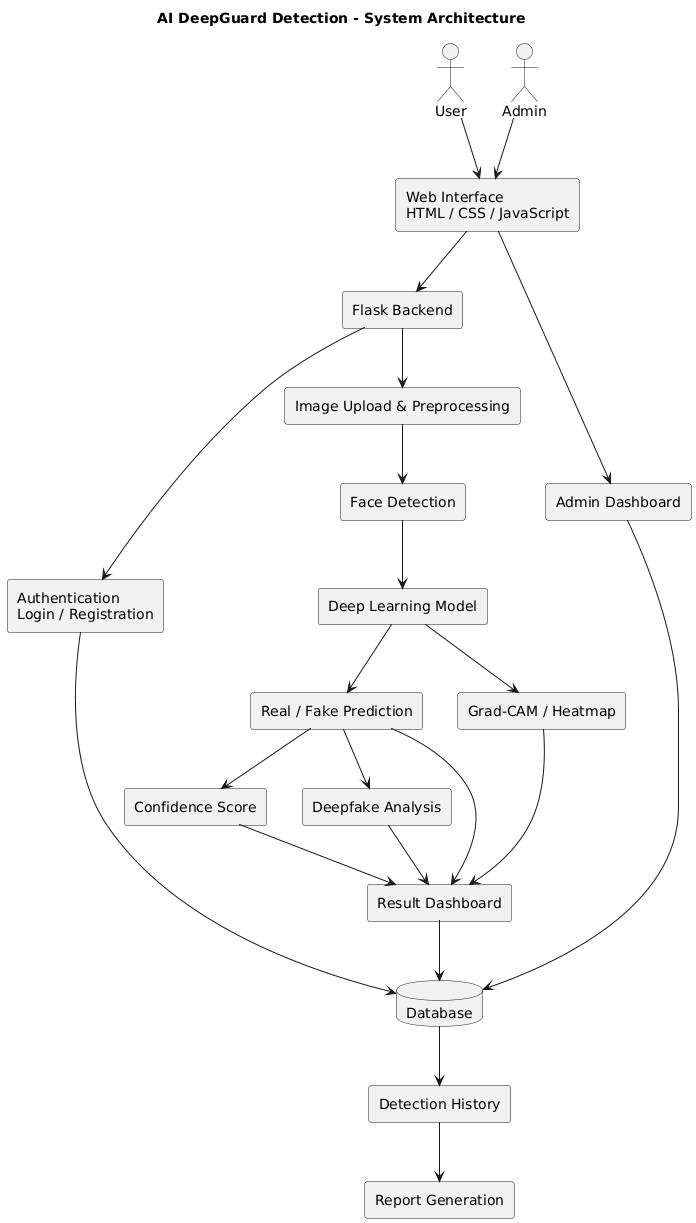
\includegraphics[
        width=\textwidth,
        height=24cm,
        keepaspectratio
    ]{deepfake.png}
    \caption{System Architecture of Ai Based Synthetic Media Detection System}
    \label{fig:architecture}
\end{figure}


% ============================================================
% CHAPTER 6
% ============================================================
\chapter{Expected Results and Discussion}

The proposed Ai Based Synthetic Media Detection System system is expected to provide an automated mechanism for identifying potentially manipulated facial images.

After uploading an image, the system is expected to detect the face and process it through the deep learning model. The final result should classify the image as either Real or Fake and display a corresponding confidence score.

The system is also expected to provide a Grad-CAM/heatmap visualization. The visualization will help identify the regions of the image that contributed significantly to the model's prediction.

The result dashboard is expected to provide a clear presentation of:

\begin{itemize}
    \item Uploaded image.
    \item Detected face.
    \item Real/Fake prediction.
    \item Confidence score.
    \item Deepfake analysis.
    \item Grad-CAM/heatmap.
    \item Detection date and time.
\end{itemize}

Detection information will be stored in the database and made available through the detection history module. Users will be able to review previous detection results and generate reports.

The administrator dashboard is expected to provide system-level monitoring of users and detection activities.

\section{Expected Performance Evaluation}

The deep learning model will be evaluated using standard classification metrics.

\begin{equation}
Accuracy =
\frac{TP + TN}{TP + TN + FP + FN}
\end{equation}

where:

\begin{itemize}
    \item $TP$ = True Positive
    \item $TN$ = True Negative
    \item $FP$ = False Positive
    \item $FN$ = False Negative
\end{itemize}

Precision, recall, and F1-score will also be considered to obtain a broader evaluation of the model.

\section{Discussion}

The proposed system is designed to combine detection accuracy with interpretability and usability. Unlike a basic classifier that only returns a binary result, Ai Based Synthetic Media Detection System provides a confidence score and visual explanation.

Grad-CAM/heatmap visualization can help users understand which facial regions contributed to the classification. This is particularly useful because deep learning models may otherwise behave as black-box systems.

The integrated database, history, report, authentication, and administration modules further improve the practical usability of the system.


% ============================================================
% CHAPTER 7
% ============================================================
\chapter{Conclusion}

Ai Based Synthetic Media Detection System proposes an AI-based web application for detecting potentially manipulated facial images. The system integrates deep learning, computer vision, explainable artificial intelligence, and web technologies into a unified platform.

The proposed system performs face detection and Real/Fake classification while providing a confidence score for the prediction. Grad-CAM and heatmap visualization are incorporated to provide an interpretable representation of the regions influencing the model's decision.

The system also includes a result dashboard, detection history, report generation, authentication, database integration, and an administrator dashboard. Flask is used for backend development, while HTML, CSS, and JavaScript are used to provide the web interface.

The proposed solution can serve as a practical academic implementation for studying deepfake detection and explainable AI. However, detection results should be interpreted as model-based assessments rather than definitive forensic proof.

Future development can extend the system toward video deepfake detection, improved cross-dataset generalization, multimodal deepfake detection, real-time analysis, additional explainability techniques, and more advanced forensic analysis.


% ============================================================
% REFERENCES
% ============================================================
\chapter*{References}
\addcontentsline{toc}{chapter}{References}

\begin{enumerate}[label={[\arabic*]},leftmargin=1cm]

\item
A. Rössler, D. Cozzolino, L. Verdoliva, C. Riess, J. Thies, and M. Nießner,
``FaceForensics++: Learning to Detect Manipulated Facial Images,''
\textit{Proceedings of the IEEE/CVF International Conference on Computer Vision (ICCV)},
pp. 1--11, 2019.

\item
L. Li, J. Bao, T. Zhang, H. Yang, D. Chen, F. Wen, and B. Guo,
``Face X-Ray for More General Face Forgery Detection,''
\textit{Proceedings of the IEEE/CVF Conference on Computer Vision and Pattern Recognition (CVPR)},
pp. 5001--5010, 2020.
DOI: 10.1109/CVPR42600.2020.00505.

\item
S. Chen, T. Yao, Y. Chen, S. Ding, J. Li, and R. Ji,
``Local Relation Learning for Face Forgery Detection,''
\textit{Proceedings of the AAAI Conference on Artificial Intelligence},
vol. 35, no. 2, pp. 1081--1088, 2021.
DOI: 10.1609/aaai.v35i2.16193.

\item
S. Tariq, S. Lee, and S. S. Woo,
``One Detector to Rule Them All: Towards a General Deepfake Attack Detection Framework,''
\textit{Proceedings of the Web Conference (WWW '21)},
pp. 3625--3637, 2021.
DOI: 10.1145/3442381.3449809.

\item
S. H. Silva, M. Bethany, A. M. Votto, et al.,
``Deepfake Forensics Analysis: An Explainable Hierarchical Ensemble of Weakly Supervised Models,''
\textit{Forensic Science International: Synergy},
vol. 4, 100217, 2022.
DOI: 10.1016/j.fsisyn.2022.100217.

\item
D. Nguyen, N. Mejri, I. P. Singh, P. Kuleshova, M. Astrid,
A. Kacem, E. Ghorbel, and D. Aouada,
``LAA-Net: Localized Artifact Attention Network for Quality-Agnostic
and Generalizable Deepfake Detection,''
\textit{Proceedings of the IEEE/CVF Conference on Computer Vision
and Pattern Recognition (CVPR)}, pp. 17395--17405, 2024.

\item
Z. Huang, J. Hu, X. Li, Y. He, X. Zhao, B. Peng, B. Wu,
X. Huang, and G. Cheng,
``SIDA: Social Media Image Deepfake Detection, Localization and
Explanation with Large Multimodal Model,''
\textit{Proceedings of the IEEE/CVF Conference on Computer Vision
and Pattern Recognition (CVPR)}, pp. 28831--28841, 2025.
DOI: 10.1109/CVPR52734.2025.02685.


\end{enumerate}


% ============================================================
% END DOCUMENT
% ============================================================
\end{document}